
 %\subsubsection{Used rules in hardware library}

This section presents the verification of modules from basic data types.
By default, AtelierB~\cite{atelierB} does not verify the type of defined functions in the clause $PROPERTIES$ from Machine. For example, the function $inc$, defined as $inc \in \{0,1\} \fun \{0,1\} \land inc = \lambda(x).( x \in \{0,1\} | x + 1)$, does not create a proof obligation to check the consistency of the definition. However, this function is not well typed because $inc(1)=2$ and $ 2 \not\in \{0,1\}$. To guarantee the type of functions, it must be declared separately: the definition of the function in $PROPERTIES$ clause and its type in the $ASSERTIONS$ clause. There are conversion functions that need to check its type. 
However, it was not possible to build proofs using the base of rules from the free distribution of AtelierB.


Another solution is to check with ProB \cite{proB}, as it is able to verify the type of functions, but its support is more suitable for finite functions. However, these functions use the concept of sequence, that is an infinite set. So a solution is to formalize rules to check these properties in AtelierB.
These created rules are assumed true hypotheses for the conversion functions and they are used in interactive prover of AtelierB. These rules also are important, because  AtelierB's prover cannot simplify easily arithmetic expressions.

The hardware library has many conversion functions with arithmetic, for example, Bit\_vector to Natural, Natural to Bit\_vector, Integer to Bit\_vector and Bit\_vector to Integer. These functions are organized in modules and each module contains auxiliary functions for a data type. The modules are represented by gray rectangles in Figure \ref{DiagramTypesRules}. %and they have the  mean: \textit{BYTE} is a bit vector with eight elements enumerated 
%starting from one; \textit{UCHAR} is a range between 0 and 255; \textit{SCHAR} is a range between -128 and 127; 
%\textit{BV16} is a bit vector with sixteen elements enumerated starting from one; \textit{USHORT} is a range 
%between 0 and 65535; and \textit{SSHORT} is a range between -32768 and 32767.

\begin{figure}[he]
\centering
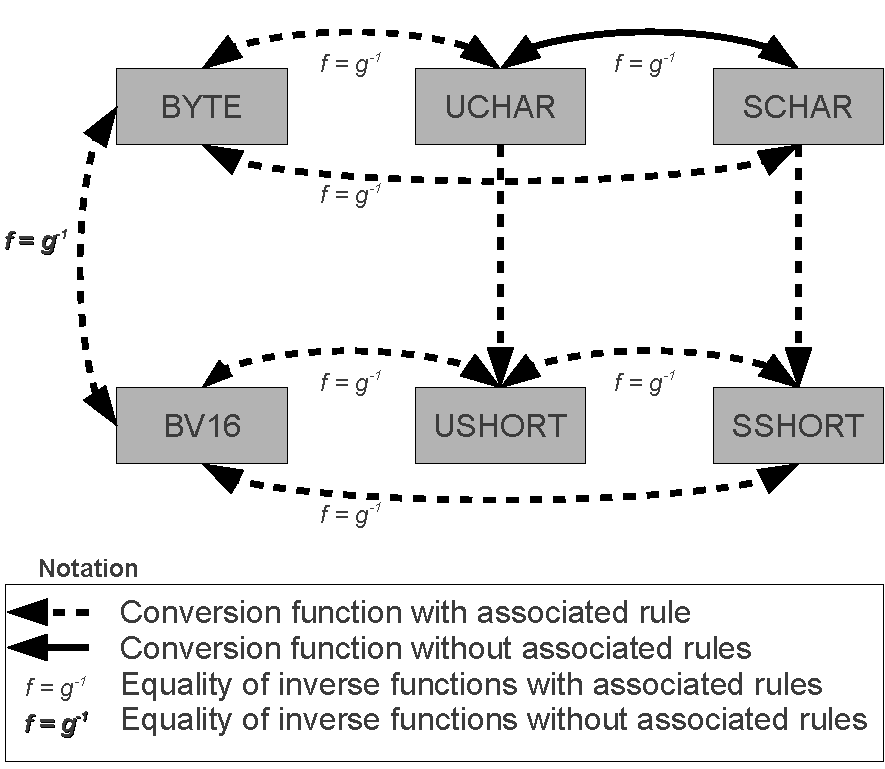
\includegraphics[width=3.in]{images/Diagram_Types_and_Rules.pdf}
\caption{Conversion functions}
\label{DiagramTypesRules}
\end{figure}


We needed to verify the type of these conversion functions. % There are twenty rules associated this properties 
Basically, these functions must keep two properties: to be bijective and equal to the reverse function.  This is not easy to verify it using AtelierB. Only three more simple proof obligations were verified automatically with the AtelierB: (\it uchar\_schar\rm \ $\in$ \textit{UCHAR} $\bij$ \textit{SCHAR}), (\it schar\_uchar\rm \ $\in$ \textit{SCHAR} $\bij$ \textit{UCHAR}) and (\it byte\_bv16\rm \ $=$ \it bv16\_byte\rm $^{-1}$).
%\begin{enumerate}
%
%\item (\it uchar\_schar\rm \ $\in$ \textit{UCHAR} $\bij$ \textit{SCHAR})
%\item (\it schar\_uchar\rm \ $\in$ \textit{SCHAR} $\bij$ \textit{UCHAR})
%\item (\it byte\_bv16\rm \ $=$ \it bv16\_byte\rm $^{-1}$) 
%
%\end{enumerate}
However, there are similar proof obligations that needed to create associated rules, in general, they are almost identical then only three are illustrated here:


%Four conditions are needed to be a bijective function:
%
%\begin{description}
%\item $func$ is a function:\\
%$\forall$ \rm (\it xx\rm ,\it yy\rm ,\it zz\rm )\rm .\rm ( \it xx  $\in$  \bf dom\rm (\it func\rm )  $\land$  \it yy $\in$  \bf ran\rm (\it func\rm )  $\land$ \\ \it zz $\in$  \bf ran\rm (\it func\rm )  $\land$ \rm ( \it xx $\mapsto$  \it yy\rm )  $\in$  \it func  $\land$  \rm ( \it xx $\mapsto$  \it zz\rm )  $\in$  \it func  $\implies$  \it yy\rm =\it zz \rm )
%
%\item $func$ is an injective function:\\
%$\forall$ \rm (\it vv\rm ,\it xx\rm )\rm .\rm ( \it vv $\in$  \bf dom\rm (\it func\rm )  $\land$  \it xx  $\in$  \bf dom\rm (\it func\rm )  $\implies$  \it func\rm (\it vv\rm )\rm =\it func\rm (\it xx\rm ) \rm )
%
%\item $func$ is a total function:\\
%$\forall$ \it xx\rm .\rm ( \it xx  $\in$  \bf dom\rm (\it func\rm )  $\implies$   $\exists$ \it yy\rm .\rm ( \it yy  $\in$  \bf ran\rm (\it func\rm )  $\land$  \it func\rm (\it xx\rm )\rm =\it yy \rm )\rm ) 
%
%\item $func$ is surjective function:\\
% $\forall$ \it yy\rm .\rm ( \it yy $\in$  \bf ran\rm (\it func\rm ) $\implies$   $\exists$ \it xx\rm .\rm ( \it xx  $\in$  \bf dom\rm (\it func\rm ) $\land$  \it func\rm (\it xx\rm )\rm =\it yy \rm )\rm ) 
%
%
%\end{description} 
%
%Here, two conversion functions between bit vectors and the natural are presented. These functions are finite and convert from \textit{BYTE} to \textit{UCHAR} and vice versa.\textit{UCHAR} is a range between 0 and 255 and \textit{BYTE} is a bit vector with eight elements enumerated starting from 1. We need to prove that $byte\_uchar$  and $uchar\_byte$  are bijective functions and  $byte\_uchar = uchar\_byte^{-1}$. These functions are defined as follows:
%\begin{description}
%
%
%\item\it byte\_uchar \rm = $\lambda$  \rm ( \it v0 \rm ) \rm . \rm ( \it v0  $\in$  \it BYTE  $\mid$ \hspace*{0.10in}\it 2$^{7}$ $\times$ \it v0\rm (\rm 8\rm )\rm +\it 2$^{6}$  $\times$ \it v0\rm (\rm 7\rm )\rm + \it 2$^{5}$ $\times$ \it v0\rm (\rm 6\rm )\rm +\it 2$^{4}$ $\times$ \it v0\rm (\rm 5\rm ) \rm + \it 2$^{3}$  $\times$  \it v0\rm (\rm 4 \rm ) \rm + \it 2$^{2}$  $\times$ \it v0\rm (\rm 3\rm ) \rm + \it 2$^{1}$  $\times$  \it v0\rm (\rm 2\rm ) \rm + \it 2$^{0}$  $\times$  \it v0\rm (\rm 1\rm )\rm) 
%
%\item\it uchar\_byte \rm = $\lambda$  \rm ( \it v0 \rm ) \rm . \rm ( \it v0  $\in$  \it UCHAR $\mid$ \rm [\rm (\it v0   $\mod$ \it 2$^{1}$\rm ) $\div$ \it 2$^{0}$\rm , \rm (\it v0  $\mod$  \it 2$^{2}$\rm ) $\div$ \it 2$^{1}$\rm , \rm (\it v0  $\mod$  \it 2$^{3}$\rm ) $\div$ \it 2$^{2}$\rm , \rm (\it v0  $\mod$  \it 2$^{4}$\rm ) $\div$ \it 2$^{3}$\rm , \rm (\it v0  $\mod$  \it 2$^{5}$\rm ) $\div$ \it 2$^{4}$\rm , \rm(\it v0  $\mod$  \it 2$^{6}$\rm ) $\div$ \it 2$^{5}$\rm ,\rm (\it v0  $\mod$  \it 2$^{7}$\rm ) $\div$ \it 2$^{6}$\rm , \rm (\it v0  $\mod$  \it 2$^{8}$\rm ) $\div$ \it 2$^{7}$\rm \rm ] \rm)
%
%\end{description}
%
%The equivalent definitions using B sequence notation and set notation are:\\
%\it uchar\_byte \rm = \rm \{ \rm 0 $\mapsto$ \rm \rm [\rm 0\rm ,\rm 0\rm ,\rm 0\rm ,\rm 0\rm ,\rm 0\rm ,\rm 0\rm ,\rm 0\rm ,\rm 0\rm \rm ]\rm, \ldots  , \rm 2\rm 5\rm 5 $\mapsto$ \rm \rm [\rm 1\rm ,\rm 1\rm ,\rm 1\rm ,\rm 1\rm ,\rm 1\rm ,\rm 1\rm ,\rm 1\rm ,\rm 1\rm \rm ]\rm \}  \\
%\it byte\_uchar \rm =  \rm \{\rm \rm [\rm 0\rm ,\rm 0\rm ,\rm 0\rm ,\rm 0\rm ,\rm 0\rm ,\rm 0\rm ,\rm 0\rm ,\rm 0\rm \rm ] $\mapsto$ \rm 0\rm, \ldots , \rm \rm [\rm 1\rm ,\rm 1\rm ,\rm 1\rm ,\rm 1\rm ,\rm 1\rm ,\rm 1\rm ,\rm 1\rm ,\rm 1\rm \rm ] $\mapsto$ \rm 2\rm 5\rm 5 \rm \} \rm 
%
%\paragraph{B Rules:}
%These rules represent that  $byte\_uchar$  and $uchar\_byte$  are bijective functions and  $byte\_uchar = uchar\_byte^{-1}$. These rules are used on interactive prover of Atelierb.



\begin{enumerate}

\item The proof obligation (\it byte\_uchar\rm \ $\in$ \textit{BYTE} $\bij$ \textit{UCHAR}) and its expansion in rule format is:\\ 
$\lambda$ \it v0\rm .\rm (\it v0 $\in$  \rm 1 $\upto$ \rm 8  $\fun$  \rm \{\rm 0\rm ,\rm 1\rm \}  $\mid$  \rm 1\rm 2\rm 8 $\times$ \it v0\rm (\rm 8\rm )\rm +\rm 6\rm 4 $\times$ \it v0\rm (\rm 7\rm )\rm +\rm 3\rm 2 $\times$ \it v0\rm (\rm 6\rm )\rm +\rm 1\rm 6 $\times$ \it v0\rm (\rm 5\rm )\rm +\rm 8 $\times$ \it v0\rm (\rm 4\rm )\rm +\rm 4 $\times$ \it v0\rm (\rm 3\rm )\rm +\rm 2 $\times$ \it v0\rm (\rm 2\rm )\rm +\rm 1 $\times$ \it v0\rm (\rm 1\rm )\rm ) \rm $\in$ \rm (\rm 1 $\upto$ \rm 8  $\fun$  \rm \{\rm 0\rm ,\rm 1\rm \}\rm )  $\bij$  \rm 0 $\upto$ \rm 2\rm 5\rm 5 \\

\item The proof obligation (\it uchar\_byte\rm \ $\in$ \textit{UCHAR} $\bij$ \textit{BYTE}) and its expansion in rule format is:\\ 
$\lambda$ \it v0\rm .\rm (\it v0 $\in$  \rm 0$\upto$255  $\mid$  \rm \rm  [(\it v0  $\mod$  \rm 2)$\div$1,(\it v0  $\mod$  \rm 4)$\div$\rm 2\rm,(\it v0  $\mod$  \rm 8)$\div$\rm 4\rm,(\it v0  $\mod$  \rm 16)$\div$\rm 8\rm,(\it v0  $\mod$  \rm 32)$\div$\rm 1\rm 6\rm,(\it v0  $\mod$  \rm 6\rm 4)$\div$\rm 3\rm 2\rm,(\it v0  $\mod$  \rm 1\rm 2\rm 8)$\div$\rm 6\rm 4\rm,(\it v0  $\mod$  \rm 2\rm 5\rm 6)$\div$\rm 1\rm 2\rm 8\rm \rm ]\rm ) \rm   $\in$  \rm 0 $\upto$ \rm 2\rm 5\rm 5   $\bij$ \rm (\rm 1 $\upto$ \rm 8  $\fun$  \rm \{\rm 0\rm ,\rm 1\rm \}\rm )\\


\item  The proof obligation (\it byte\_uchar\rm  =  \it uchar\_byte\rm$^{-1}$) and its expansion in rule format is:\\ 
  $\lambda$ \it v0\rm .\rm (\it v0 $\in$  \rm 1 $\upto$ \rm 8  $\fun$  \rm \{\rm 0\rm ,\rm 1\rm \}  $\mid$  \rm 1\rm 2\rm 8 $\times$ \it v0\rm (\rm 8\rm )\rm +\rm 6\rm 4 $\times$ \it v0\rm (\rm 7\rm )\rm +\rm 3\rm 2 $\times$ \it v0\rm (\rm 6\rm )\rm +\rm 1\rm 6 $\times$ \it v0\rm (\rm 5\rm )\rm +\rm 8 $\times$ \it v0\rm (\rm 4\rm )\rm +\rm 4 $\times$ \it v0\rm (\rm 3\rm )\rm +\rm 2 $\times$ \it v0\rm (\rm 2\rm )\rm +\rm 1 $\times$ \it v0\rm (\rm 1\rm )\rm )=($\lambda$ \it v0\rm .\rm (\it v0 $\in$  \rm 0$\upto$255  $\mid$  \rm \rm  [(\it v0  $\mod$  \rm 2)$\div$1,(\it v0  $\mod$  \rm 4)$\div$\rm 2\rm,(\it v0  $\mod$ \rm 8) $\div$\rm 4\rm,(\it v0  $\mod$  \rm 16)$\div$\rm 8\rm,(\it v0  $\mod$  \rm 32)$\div$\rm 1\rm 6\rm,(\it v0  $\mod$ \rm 6\rm 4)$\div$\rm 3\rm 2\rm,(\it v0  $\mod$  \rm 1\rm 2\rm 8)$\div$\rm 6\rm 4\rm,(\it v0  $\mod$  \rm 2\rm 5\rm 6)$\div$\rm 1\rm 2\rm 8\rm \rm ]\rm )\rm)$^{-1}$
\end{enumerate}

Other four proof obligations are using rules to demonstrated that the functions
are finite: \it byte\_uchar  $ \in \finset$\rm (\it byte\_uchar\rm ); \it
uchar\_byte  $ \in \finset$\rm (\it uchar\_byte\rm ); \it ushort\_bv16 $ \in
\finset$\rm (\it ushort\_bv16\rm ) and \it bv16\_ushort $ \in \finset$\rm (\it
bv16\_ushort\rm ).
\begin{enumerate}
\item  The proof obligation (\it byte\_uchar $\in$   $\finset$ \rm (\it byte\_uchar\rm )) and its expansion in rule format is:\\ 
 $\lambda$ \it v0\rm .\rm (\it v0 $\in$  \rm 1 $\upto$ \rm 8  $\fun$  \rm \{\rm 0\rm ,\rm 1\rm \}  $\mid$  \rm 1\rm 2\rm 8 $\times$ \it v0\rm (\rm 8\rm )\rm +\rm 6\rm 4 $\times$ \it v0\rm (\rm 7\rm )\rm +\rm 3\rm 2 $\times$ \it v0\rm (\rm 6\rm )\rm +\rm 1\rm 6 $\times$ \it v0\rm (\rm 5\rm )\rm +\rm 8 $\times$ \it v0\rm (\rm 4\rm )\rm +\rm 4 $\times$ \it v0\rm (\rm 3\rm )\rm +\rm 2 $\times$ \it v0\rm (\rm 2\rm )\rm +\rm 1 $\times$ \it v0\rm (\rm 1\rm )\rm ) $\in$   $\finset$ \rm ( $\lambda$ \it v0\rm .\rm (\it v0 $\in$  \rm 1 $\upto$ \rm 8  $\fun$  \rm \{\rm 0\rm ,\rm 1\rm \}  $\mid$  \rm 1\rm 2\rm 8 $\times$ \it v0\rm (\rm 8\rm )\rm +\rm 6\rm 4 $\times$ \it v0\rm (\rm 7\rm )\rm +\rm 3\rm 2 $\times$ \it v0\rm (\rm 6\rm )\rm +\rm 1\rm 6 $\times$ \it v0\rm (\rm 5\rm )\rm +\rm 8 $\times$ \it v0\rm (\rm 4\rm )\rm +\rm 4 $\times$ \it v0\rm (\rm 3\rm )\rm +\rm 2 $\times$ \it v0\rm (\rm 2\rm )\rm +\rm 1 $\times$ \it v0\rm (\rm 1\rm )\rm )\rm )  \\


\end{enumerate}


So there are in total twenty four rules related to binary arithmetic.These rules
are used to facilitate the manipulation of theorem prover with binary arithmetic
developed by \cite{Leibnizens}. They guarantee important properties that are
demonstrated in \cite{James2010,Dasgupta2006}. The others proof obligations with
associated rule are very similar, they have just small differences, for example,
the size of bit vectors.











%
%To guarantee these rules, a demonstration will be shown. We need verify if (\it byte\_uchar\rm \ $\in$ \textit{BYTE} $\bij$ \textit{UCHAR}) then four conditions must be verified.
%
%Is $byte\_uchar$ a function ?\\
%\begin{tabular}{l c}
%$\forall$ \rm (\it xx\rm ,\it yy\rm ,\it zz\rm )\rm .\rm ( \it xx  $\in$  \bf dom\rm (\it byte\_uchar\rm )  $\land$  \it yy $\in$  \bf ran\rm (\it byte\_uchar\rm  )  \\
%$\land$  \it zz $\in$  \bf ran\rm (\it byte\_uchar\rm )  $\land$ \rm ( \it xx $\mapsto$  \it yy\rm )  $\in$  \it byte\_uchar\rm  $\land$\\
%\rm ( \it xx $\mapsto$  \it zz\rm )  $\in$  \it byte\_uchar\rm   $\implies$  \it yy\rm =\it zz \rm )\\\\
%\end{tabular}
%\\
%Step 1 - Replacing the sets:\\
%\begin{tabular}{l c}
%$\forall$ \rm (\it xx\rm ,\it yy\rm ,\it zz\rm )\rm .\rm ( \it xx  $\in$  \it BYTE\rm  $\land$  \it yy $\in$  \it UCHAR\rm $\land$  \it zz $\in$  \it UCHAR \rm  \\
%$\land$ \rm ( \it xx $\mapsto$  \it yy\rm )  $\in$  \it byte\_uchar \rm  $\land$ \rm ( \it xx $\mapsto$  \it zz\rm )  $\in$  \it byte\_uchar\rm  $\implies$  \it yy\rm =\it zz \rm )\\\\
%\end{tabular}
%\\
%Step 2 - Expanding \it byte\_uchar \rm and replacing the sets:\\
%\begin{tabular}{l c}
%$\forall$ \rm (\it xx\rm ,\it yy\rm ,\it zz\rm )\rm .\rm ( \it xx  $\in$  \it BYTE \rm  $\land$  \it yy $\in$  \it UCHAR \rm $\land$  \it zz $\in$  \it UCHAR \rm  $\land$ & {\LARGE \checkmark} \\
%\rm ( \it xx $\mapsto$  \it yy\rm ) $\in$  \rm \{\rm \rm [\rm 0\rm ,\rm 0\rm ,\rm 0\rm ,\rm 0\rm ,\rm 0\rm ,\rm 0\rm ,\rm 0\rm ,\rm 0\rm \rm ] $\mapsto$ \rm 0\rm, \ldots , \rm \rm [\rm 1\rm ,\rm 1\rm ,\rm 1\rm ,\rm 1\rm ,\rm 1\rm ,\rm 1\rm ,\rm 1\rm ,\rm 1\rm \rm ] $\mapsto$ \rm 2\rm 5\rm 5 \rm \} \rm  $\land$ \\
%\rm ( \it xx $\mapsto$  \it zz\rm ) $\in$  \rm \{\rm \rm [\rm 0\rm ,\rm 0\rm ,\rm 0\rm ,\rm 0\rm ,\rm 0\rm ,\rm 0\rm ,\rm 0\rm ,\rm 0\rm \rm ] $\mapsto$ \rm 0\rm, \ldots , \rm \rm [\rm 1\rm ,\rm 1\rm ,\rm 1\rm ,\rm 1\rm ,\rm 1\rm ,\rm 1\rm ,\rm 1\rm ,\rm 1\rm \rm ] $\mapsto$ \rm 2\rm 5\rm 5 \rm \} \rm  $\implies$  \it yy\rm =\it zz \rm )\\\\
%\end{tabular}
%
%
%
%Is $byte\_uchar$ an injective function?\\
%\begin{tabular}{l c}
%$\forall$ \rm (\it vv\rm ,\it xx\rm )\rm .\rm ( \it vv $\in$  \bf dom\rm (\it byte\_uchar\rm )  $\land$  \it xx  $\in$  \bf dom\rm (\it byte\_uchar\rm) & {\LARGE \checkmark} \\
% $\implies$  \it byte\_uchar\rm (\it vv\rm )\rm =\it byte\_uchar\rm (\it xx\rm ) \rm )\\\\
%\end{tabular}
%
%Is $byte\_uchar$ a total function?\\
%\begin{tabular}{l c}
%$\forall$ \it xx\rm .\rm ( \it xx  $\in$  \bf dom\rm (\it byte\_uchar\rm )  $\implies$ & {\LARGE \checkmark} \\
%$\exists$ \it yy\rm .\rm ( \it yy  $\in$  \bf ran\rm (\it byte\_uchar\rm )  $\land$  \it byte\_uchar\rm (\it xx\rm )\rm =\it yy \rm )\rm ) \\\\
%\end{tabular}
%
%Is $byte\_uchar$ a surjective function? \\
%\begin{tabular}{l c}
%$\forall$ \it yy\rm .\rm ( \it yy $\in$  \bf ran\rm (\it byte\_uchar\rm  ) $\implies$ & {\LARGE \checkmark} \\
%$\exists$ \it xx\rm .\rm ( \it xx  $\in$  \bf dom\rm (\it byte\_uchar\rm  ) $\land$  \it byte\_uchar\rm  (\it xx\rm )\rm =\it yy \rm )\rm ) \\\\
%\end{tabular}
%
%
%We need verify if (\it uchar\_byte\rm \ $\in$ \textit{UCHAR} $\bij$ \textit{BYTE}) then four conditions must be verified.
%
%Is $uchar\_byte$ a function ?\\
%\begin{tabular}{l c}
%$\forall$ \rm (\it xx\rm ,\it yy\rm ,\it zz\rm )\rm .\rm ( \it xx  $\in$  \bf dom\rm (\it uchar\_byte\rm )  $\land$  \it yy $\in$  \bf ran\rm (\it uchar\_byte\rm  )& {\LARGE \checkmark} \\
%$\land$  \it zz $\in$  \bf ran\rm (\it uchar\_byte\rm )  $\land$ \rm ( \it xx $\mapsto$  \it yy\rm )  $\in$  \it uchar\_byte\rm  $\land$\\
%\rm ( \it xx $\mapsto$  \it zz\rm )  $\in$  \it uchar\_byte\rm   $\implies$  \it yy\rm =\it zz \rm )\\\\
%\end{tabular}
%
%Is $uchar\_byte$ an injective function?\\
%\begin{tabular}{l c}
%$\forall$ \rm (\it vv\rm ,\it xx\rm )\rm .\rm ( \it vv $\in$  \bf dom\rm (\it uchar\_byte\rm )  $\land$  \it xx  $\in$  \bf dom\rm (\it uchar\_byte\rm) & {\LARGE \checkmark} \\
% $\implies$  \it uchar\_byte\rm (\it vv\rm )\rm =\it uchar\_byte\rm (\it xx\rm ) \rm )\\\\
%\end{tabular}
%
%Is $uchar\_byte$ a total function?\\
%\begin{tabular}{l c}
%$\forall$ \it xx\rm .\rm ( \it xx  $\in$  \bf dom\rm (\it uchar\_byte\rm )  $\implies$ & {\LARGE \checkmark} \\
%$\exists$ \it yy\rm .\rm ( \it yy  $\in$  \bf ran\rm (\it uchar\_byte\rm )  $\land$  \it uchar\_byte\rm (\it xx\rm )\rm =\it yy \rm )\rm ) \\\\
%\end{tabular}
%
%Is $uchar\_byte$ a surjective function? \\
%\begin{tabular}{l c}
%$\forall$ \it yy\rm .\rm ( \it yy $\in$  \bf ran\rm (\it uchar\_byte\rm  ) $\implies$ & {\LARGE \checkmark} \\
%$\exists$ \it xx\rm .\rm ( \it xx  $\in$  \bf dom\rm (\it uchar\_byte\rm  ) $\land$  \it uchar\_byte\rm  (\it xx\rm )\rm =\it yy \rm )\rm ) \\\\
%\end{tabular}
%
%The $byte\_uchar$  and $uchar\_byte$  are bijective functions consequently each one has an inverse function, but is $byte\_uchar = uchar\_byte ^{-1}$  true ?\\
%
%$\forall$ \rm (\it xx\rm ,\it yy\rm )\rm .\rm ( \it xx  $\in$  \it UCHAR\rm   $\land$  \it yy $\in$  \it BYTE \rm   $\implies$ \\
%\rm ( \it xx $\mapsto$  \it yy\rm )  $\in$  $byte\_uchar$   $\land$  \rm ( \it yy $\mapsto$  \it xx\rm )  $\in$  $uchar\_byte$ ) \\
%
%Step 1 - Expanding \it byte\_uchar \rm  and \it uchar\_byte \rm \\\\
%\begin{tabular}{l c}
%$\forall$ \rm (\it xx\rm ,\it yy\rm )\rm .\rm ( \it xx  $\in$  \it UCHAR\rm   $\land$  \it yy $\in$  \it BYTE \rm   $\implies$  & {\LARGE \checkmark} \\
%\rm ( \it xx $\mapsto$  \it yy\rm )  $\in$  \rm \{ \rm 0 $\mapsto$ \rm \rm [\rm 0\rm ,\rm 0\rm ,\rm 0\rm ,\rm 0\rm ,\rm 0\rm ,\rm 0\rm ,\rm 0\rm ,\rm 0\rm \rm ] \rm , \ldots  , \rm 2\rm 5\rm 5 $\mapsto$ \rm \rm [\rm 1\rm ,\rm 1\rm ,\rm 1\rm ,\rm 1\rm ,\rm 1\rm ,\rm 1\rm ,\rm 1\rm ,\rm 1\rm \rm ]\rm \}  $\land$ \\
%\rm ( \it yy $\mapsto$  \it xx\rm )  $\in$  \rm \{\rm \rm [\rm 0\rm ,\rm 0\rm ,\rm 0\rm ,\rm 0\rm ,\rm 0\rm ,\rm 0\rm ,\rm 0\rm ,\rm 0\rm \rm ] $\mapsto$ \rm 0 \rm , \ldots , \rm \rm [\rm 1\rm ,\rm 1\rm ,\rm 1\rm ,\rm 1\rm ,\rm 1\rm ,\rm 1\rm ,\rm 1\rm ,\rm 1\rm \rm ] $\mapsto$ \rm 2\rm 5\rm 5\rm \} \rm ) \\ \\ 
%\end{tabular}


%
%
%% Conclusão
%\subsection{Final considerations }
%%\subsection{Considerações finais sobre o estudo de caso}
%
%%[Importáncia de ser o primeiro modelo 1° utilizando as bibliotecas]%[Completamente suportado pelo método B, principalmente devido ao uso de funções que convertem as representações dos sistemas de numeração]
%%[A importáncia das técnicas e a experiência adquirida]
%%[Explicar como pode ser útil para avaliar a vazão]
%%[ Finalmente, argumento mais importante : A técnica está sendo viabilizada,
%% pois o maior custo do processo está diminuindo devido aos avanços do atelierb e as técnicas descobertas  ]
%
%
%The \textit{TestCalc\_basm} model was the first developed model according to
%the proposal of \cite{Dantas_SBMF08} using the hardware and integer libraries. These
%libraries contain type definitions, functions and lemmas that
%could establish the relation between the B assembly model and its more
%abstract model. These definitions kept the signature of operations relating to 
%the B abstract model and the B assembly model; these simplified the
%verification process and become more faithful to the representation of
%microcontroller, everything without the need to extend the B method.
%
%% % [Importáncia do 1° modelo]
%% O modelo \textit{TestCalc\_basm} foi o primeiro construído de acordo com a proposta de [Dantas et al.
%% 2008]  utilizando as bibliotecas de \textit{hardware} e tipos inteiros. Essas bibliotecas contêm tipos,
%% funções e lemas que possibilitaram estabelecer a relação entre o modelo B \textit{assembly} e o modelo
%% mais abstrato. Essas definições mantiveram a assinatura das operações do modelo abstrato com relação ao B
%% \textit{assembly}, simplificaram o processo de verificação e tornaram mais fiel a representação do
%% microcontrolador, tudo isso sem a necessidade de estender o método B.
%
%The development of this model was too much important to improve the verification
%process, because the development and verification help the design to get new
%experiences with theorem prover (manual and interactive) and find proof
%commands\footnote{The proof commands are steps that direct the prover to find the
%proof, and cannot introduce false hypothesis.} that reduce too much the proof
%process time. These experiences become the development and verification up to
%assembly more feasible, mainly, because the most of the proof commands are
%generic. So, these proof commands can be used again in several similar proof
%obligations. In addition, the specification pattern used helps to model new and
%different platforms.
%
%% % [A importáncia das técnicas e a experiência adquirida]
%% A elaboração desse modelo foi muito importante para amadurecer o processo de verificação, pois a
%% construção e verificação do modelo ajudou ao projetista adquirir experiências com o provador interativo e
%% a descobrir comandos de prova que reduzem significativamente o tempo do processo de prova. Essa
%% experiência torna mais viável a especificação de outros \textit{softwares} mais complexos, pois a
%% maioria dos comandos de provas podem ser usados novamente em obrigações de prova similares e o padrão de
%% especificação utilizado ajuda na modelagem de novas plataformas. 
%
%%No entanto, esse mesmo \textit{software} poderia ser acoplado em dispositivo \textit{timer} e 
%%pois de forma bem eficiente foi resolvida  
%%Certamente reduzem bastante o custo de verificação,
%%pois o projetista desse modelo compreendeu a construção do invariante para linguagens assembly, 
%%é possível aproveitar as caractéristicas das provas interativas para realizar algum tipo de automação nessa etapa,
%%tudo indica que a construção da cláusula invariante pode ser feita por um algorítmo simples e    
%%[Explicar como pode ser util para avaliar a vazão] ]
%%Poderia se avaliando através da vazão, mas a modelagem ainda suporta bem aspectos temporais, por outro lado,
%%utilizando-se de um dispotivo \textit{timer} esse mesmo \textit{software} poderia calcular o tempo de enchimento do tanque
%%a vazão pode ser 
%
%Finally, the developed embedded software can work like a redundant system and it
%could provide a better confidence and quality, because the responsible engineer
%has one more way to analyse the production test and more warranties. So, the
%system can also improve the effectiveness of the test, because less failed tests
%happen.
%
%% %[ Importáncia para área de petróleo e gás ] Finalmente, o funcionamento do
%% \textit{software} desenvolvido como um sistema redudante deve oferecer uma
%% melhor confiança e qualidade, pois o engenheiro responsável terá mais um meio
%% de comparação dos testes de produção e mais garantias. Essas garantias devem-se
%% Ã  existência de um sistema redundante e a sua verificação formal até um dos
%% últimos níveis de representação do \textit{software}. Logo, o sistema pode
%% também melhorar a eficácia dos testes, visto que menos testes falhos podem
%% existir.
%
